%%%%%%%%%%%%%%%%%%%%%%%%%%%%%%%%%%%%%%%%%
% University/School Laboratory Report
% LaTeX Template
% Version 3.1 (25/3/14)
%
% This template has been downloaded from:
% http://www.LaTeXTemplates.com
%
% Original author:
% Linux and Unix Users Group at Virginia Tech Wiki 
% (https://vtluug.org/wiki/Example_LaTeX_chem_lab_report)
%
% License:
% CC BY-NC-SA 3.0 (http://creativecommons.org/licenses/by-nc-sa/3.0/)
%
%%%%%%%%%%%%%%%%%%%%%%%%%%%%%%%%%%%%%%%%%

%----------------------------------------------------------------------------------------
%	PACKAGES AND DOCUMENT CONFIGURATIONS
%----------------------------------------------------------------------------------------

\documentclass[10pt,oneside,slovak,a4paper]{article}

\usepackage{graphicx} % Required for the inclusion of images
\usepackage{amsmath} % Required for some math elements 
\usepackage[utf8]{inputenc}
\usepackage[slovak]{babel}
\usepackage{listings}
\usepackage{indentfirst}
\usepackage{float}
\usepackage{fancyhdr}
\usepackage{enumitem}
\usepackage[a4paper, total={6in, 8in}]{geometry}
\usepackage[table,xcdraw]{xcolor}
\usepackage{verbatim}
\usepackage{titling}
\usepackage{hyperref}
%\usepackage{rotating} %PRIDANY PACKAGE
%\usepackage{booktabs} %PRIDANY PACKAGE
%\usepackage{multirow}%PRIDANY PACKAGE
%\usepackage{afterpage}
%\usepackage{lipsum}
\usepackage{minted}

\pagestyle{fancy}


\graphicspath{ {./images/} }
%\pagestyle{myheadings}

\setlength{\droptitle}{-5ex} %posunutie Nazvu autora a pod vyssie

\fancypagestyle{plain}{%
   \fancyhf{} 
   \fancyfoot[C]{\tiny  Autor predlohy : Linux and Unix Users Group at Virginia Tech Wiki. Názov predlohy : University/School Laboratory Report. Predloha dokumentu licencovaná pod CC BY-NC-SA 3.0 (http://creativecommons.org/licenses/by-nc-sa/3.0/).}
   \renewcommand{\headrulewidth}{0pt}
}

%\usepackage{times} % Uncomment to use the Times New Roman font

%----------------------------------------------------------------------------------------
%	DOCUMENT INFORMATION
%----------------------------------------------------------------------------------------

\title{\textsc{Mobilné technológie a aplikácie}\\ Dokumentácia k zadaniu} % Title

\author{Lukáš \textsc{Štrbo}} % Author name

\date{1. marec 2022}
%\date{\today} % Date for the report

\author{Lukáš \textsc{Štrbo}\\[2pt]
	{\small Slovenská technická univerzita v Bratislave}\\
	{\small Fakulta informatiky a informačných technológií}\\
	{\small \texttt{xstrbol@stuba.sk}}\\
{\small \texttt{ID: 110903}}\\
	}


\begin{document}

\maketitle % Insert the title, author and date

\begin{center}
\begin{tabular}{l r}
Zadanie č. 1 : & SIP Proxy (telefónna ústredňa)\\ 
Cvičiaci: & Ing. Marek Galinski, PhD.
\end{tabular}
\end{center}

\tableofcontents
\newpage

\section{Zadanie}
Sprevádzkovanie SIP Proxy, ktorá umožní prepájanie a realizáciu hovorov medzi štandardnými SIP klientami.

Na implementáciu SIP Proxy si môžete zvoliť akýkoľvek programovací jazyk a použiť akúkoľvek SIP knižnicu, ktorá pre daný programovací jazyk existuje. Vo výsledku však musíte spúšťať “váš kód”, v ktorom sú zakomponované knižnice, ktoré poskytujú funkcionalitu SIP Proxy. Hovor musí byť realizovaný medzi dvomi fyzickými zariadeniami v rámci LAN siete


\textbf{Povinné funkcionality}
\begin{enumerate}[label=(\alph*)]
	\item Registrácia účastníka (bez nutnosti autentifikácie) 
	\item Vytočenie hovoru a zvonenie na druhej strane 
	\item Prijatie hovoru druhou stranou, fungujúci hlasový hovor 
	\item Ukončenie hlasového hovoru (prijatého aj neprijatého) 
\end{enumerate}


\textbf{Doplnkové funkcionality}
\begin{enumerate}[label=(\alph*)]
	\item Možnosť zrealizovať konferenčný hovor (aspoň 3 účastníci) 
	\item Možnosť presmerovať hovor 
	\item Možnosť realizovať videohovor 
	\item Logovanie “denníka hovorov”
	\item Úprava SIP stavových kódov v zdrojovom kóde proxy
\end{enumerate}


\section{Implementačné prostredie a repozitáre}
\label{impl}
\begin{enumerate}
	\item \textbf{Repozitáre}
	\begin{itemize}
		\item \textbf{Použitá SIP knižnica:} \url{https://github.com/tirfil/PySipFullProxy}
		\item \textbf{Osobný repozitár:} \url{https://github.com/LukasStrbo/MTAA_Sip_Proxy}
	\end{itemize}
	\item \textbf{Implementačné prostredie}
	\begin{itemize}
		\item \textbf{IDE:} PyCharm 2021.3.2 (Professional Edition)
		\item \textbf{Programovací jazyk:} Python 3.9.7
		\item \textbf{OS:} Microsoft Windows 10 [Version 10.0.19043.1526]
		\item \textbf{Klient:} Linphone 
	\end{itemize}
\end{enumerate}

\section{Riešenie zadania}
\subsection{Implementácia riešenia}
Riešenie bolo implementované pomocou SIP knižnice z platformy GitHub (viď. \ref{impl}). SIP knižnica bola pravdepodobne naprogramovaná pre staršiu verziu programovacieho jazyka Python nakoľko po jej spustení sa vyskytli rôzne výnimky a chyby. Pre to bolo potrebné danú knižnicu opraviť a prispôsobiť ju novým štandardom novšej verzie progamovacieho jazyka Python.

\subsection{Povinné funkcionality}
PRe spojazdnenie povinných funkcionalít bola potrebná oprava SIP knižnice. Knižnica vykazovala po spustení isté výnimky a chyby. Chyby, ktoré boli v knižnici spôsobené boli hlavne spôsobené tým, že knižnica bola programovaná v staršej verzii jazyka Python.

Opravené chyby v knižnici:
\begin{itemize}
	\item Pri posielaní dát boli posielané datové typy \textbf{string} a nie \textbf{byte}
	\item Stará forma použitia príkazu join pre stringy
	\item Stará forma použitia kontroly nachádzajúceho sa kľúca v poli (z \textbf{X.has\_key(Y)} na \textbf{Y in X})
\end{itemize}

\subsection{Doplnkové funkcionality}
\subsubsection{Úprava SIP stavových kódov}
Na úpravu stavových kódov bolo potrebné pochopiť akým spôsobom sú kódy na SIP Proxy spracúvané.
\begin{figure}[H]
	\label{flow1}
	\centering
	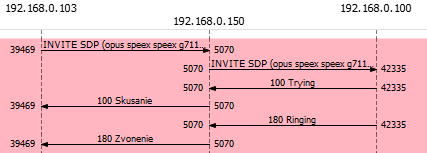
\includegraphics[scale=1, width=\textwidth]{chart1.png}
	\caption{Okresaný flowchart hovoru medzi dvoma účasntikmi hovoru}
\end{figure}

Ak sa pozrieme na odchytené packety a následne na Call Flow poskytnutý programom Wireshark môžeme na obrázku \ref{flow1} vidieť začiatok vyzvánania. Jedna strana pošle cez server druhej strane \textbf{INVITE}, ktorý následne spustí sekvenciu dvoch SIP kódov od druhej strany - \textbf{100 Trying, 180 Ringing}. Na grafe je možné vidieť, že SIP komunikácia prebieha tak, že všetky požiadavky a kódy idú cez SIP Proxy Server.

Pre to aby sme dokázali zmeniť, kódy potrebujeme upraviť knižnicu a prísť na to kde sa tieto kódy spracúvajú.

\newpage
Okresaný a zjednodušený kód knižnice:
\begin{minted}[fontsize=\footnotesize, mathescape, linenos, numbersep=5pt, frame=lines, framesep=2mm]{python}
rx_request_uri = re.compile("^([^ ]*) sip:([^ ]*) SIP/2.0")
rx_code = re.compile("^SIP/2.0 ([^ ]*)")
 
class UDPHandler(socketserver.BaseRequestHandler):
	def processCode(self):
		# Kod funkcie

	def processRequest(self):
		if len(self.data) > 0:
			request_uri = self.data[0]
			# If strom kontroly regexov
			if ...:
				
			elif ...:

			elif rx_code.search(request_uri):
				self.processCode() 

	def handle(self):
		self.data = data.split("\r\n")
		request_uri = self.data[0]
		if rx_request_uri.search(request_uri) or rx_code.search(request_uri):
		self.processRequest()
\end{minted}

Kód knižnice je postavený na základe spracovávania všetkých požiadaviek pomocou funckie \textbf{handle()}, ktorá pomocou reg-ex výrazov zistí, či sa jedná o SIP požiadavku. Ak áno prejde sa do funckie \textbf{processRequest()}, ktorá skontroluje pomocou ďalších reg-ex výrazov o akú SIP požiadavku / správu sa jedná. Tu môžeme vidieť, že existuje rexgex výraz, ktorý kontroluje SIP stavové kódy a volá sa funckcia \textbf{processCode()}

Táto funckia spracováva všetky SIP stavové kódy. V tejto funckii bude potrebné tieot správy upravovať.

Okresaný a zjednodušený kód funkcie \textbf{processCode()}:
\begin{minted}[fontsize=\footnotesize, mathescape, linenos, numbersep=5pt, frame=lines, framesep=2mm]{python}
    def processCode(self):
        origin = self.getOrigin()
        if len(origin) > 0:
            if origin in registrar:
                socket, claddr = self.getSocketInfo(origin)
                self.data = self.removeRouteHeader()
                data = self.removeTopVia()

		# #############################
		# Vlastny kod na vymenu SIP stavovych kodovsprav
                for key in code_messages:
                    check_msg = "SIP/2.0 " + key
                    if data[0] == check_msg:
                        data[0] = "SIP/2.0 " + code_messages[key]
                        break
		# #############################
                text = "\r\n".join(data)
                socket.sendto(text.encode(), claddr)
\end{minted}

Vlastný kód prezrie string, ktorý obsahuje SIP stavový kód spoločne s jeho správou a na základe externého súboru \textbf{check\_msg.json}.

\subsubsection{Denník hovorov}
Denník hovor funguje na základe spracovácania požiadaviek serverom. Akonáhle je požiadavka pre server SIP požiadavka zavolá sa vlastná funkcia \textbf{call\_log(data)}, ktorá spracuje požiadavku a pozrie sa na jej obsah na základe ktorej rozhodne či sa jedná o hovor.

Hlavné časti kódu spracovnia denníka hovorov:
\begin{minted}[fontsize=\footnotesize, mathescape, linenos, numbersep=5pt, frame=lines, framesep=2mm]{python}
rx_ringing = re.compile("^SIP/2.0 180.*")
rx_decline = re.compile("^SIP/2.0 603.*")
rx_ok = re.compile("^SIP/2.0 200.*")
rx_terminated = re.compile("^SIP/2.0 487.*")
rx_busy_here = re.compile("^SIP/2.0 486.*")
rx_bye = re.compile("^BYE")

class CallLog:  
	# Trieda CallLog - Pre kazdy individualny hovor samostatny objekt
    call_id = ""
    fromm = ""
    to = ""
    start_ring = None
    start = None
    end = None
    status = ""

    def __init__(self, call_id, fromm, to, start_ring):
        self.fromm = fromm
        self.to = to
        self.start_ring = start_ring
        self.call_id = call_id

def call_log(data):
	# Funkcia, ktora spracuje poziadavku na zaklade CallID
    # Najdenie CALL-ID z prichodzich dat a vytvorneie premennej log
    if rx_ringing.search(req_uri):  # Ak niekto zacal volat a zvoni
        # Vytvorenie objektu CallLog na zaklade CallID
	elif log: # kontrola existenie dennika pre CallID
		if rx_decline.search(req_uri):  # Odmietnutie hovoru
			# Zapisanie do suboru
		elif rx_terminated.search(req_uri):  # Zrusenie zvoenia volajucim
			# Zapisanie do suboru
		elif rx_busy_here.search(req_uri):  # Neodpovedanie
			# Zapisanie do suboru
		elif rx_bye.search(req_uri):  # Ukoncenie hovoru
			# Zapisanie do suboru
		elif rx_ok.search(req_uri):  # Zaciatok telefonovania po zdvihnuti
			# Zapisanie casu zaciatku hovoru
\end{minted}

Zjendoduseny kod spracovania dennika hovoru v triede spracovania SIP požiadaviek:
\begin{minted}[fontsize=\footnotesize, mathescape, linenos, numbersep=5pt, frame=lines, framesep=2mm]{python}
class UDPHandler(socketserver.BaseRequestHandler):
	def processRequest(self):
        	if len(self.data) > 0:
            	request_uri = self.data[0]
            	call_log(self.data)  # Dennik hovorov - Vlastna Funkcia

			# IF-ELSE Strom pre konkretnu poziadavku na zklade Reg-EX
\end{minted}

\subsection{Zhrnutie funkcionality}
Na testovanie funkcionality SIP Proxy servera bol použitý klient \textbf{Linphone}. SIP Proxy server dokáže registrovať účastníkov bez nutnosti autentifikácie a sprostredkovať hovor medzi dvoma účastníkmi so všetkými funkcionalitami ako vyzvánanie, zrušenie hovoru, podržanie hovoru ale aj chat. Funkčné je aj ak účastník hovor odmietne alebo ak volájúci sa rozhodne na volané číslo prestať volať ešte v momente keď hovor nebol zdvihnutý. Je možné vykonať aj konferenčný hovor, ktorý bol otestovaný medzi 3ma účastnikmi. Úspešné bolo aj vykonanie videohovoru a presmerovanie hovoru spoločne s podržaním účasntíka, ktorý tento hovor presmeroval. 

Doplnkovou funkcionalitou je aj logovanie denníka hovorov a úprava stavových SIP kódov. Logovanie zaznamenáva všetky hovory, ktoré boli zdvihnuté, zamietnuté alebo zamietnuté volajúcim. Logovanie poksytuje aj záznam konferenčného hovoru s tým, že v denníku sa takýto hovor zobrazuje ako dva rozdiele hovory medzi účastníkmi. Mimo iné denník zaznamená stav hovoru (ukončený, odmietnutý, odmietnutý volajúcim) a zároveň čas odkedy volajúci začal volať, čas zdvihnutia a čas ukončenia hovoru.

Doplnkové funkcionality ako videohovor, presmerovanie hovoru a konferenčný hovor už boli podporované použitou SIP knižnicou a klientom.
%\thispagestyle{fancy}

\section{Opis SIP Komunikácie}
\subsection{Odmietnutie, zrušenie, hovor}
Pozrieme sa na záznam paketov z troch scenárov medzi dvoma klientami. Jedná sa normálne vyzváňanie avšak jeden z nich je odmietnutý druhou stranou, ďalší je zrušený volajúcim a posledný je normálny hovor s klasickým ukončením.

\begin{figure}[H]
	\centering
	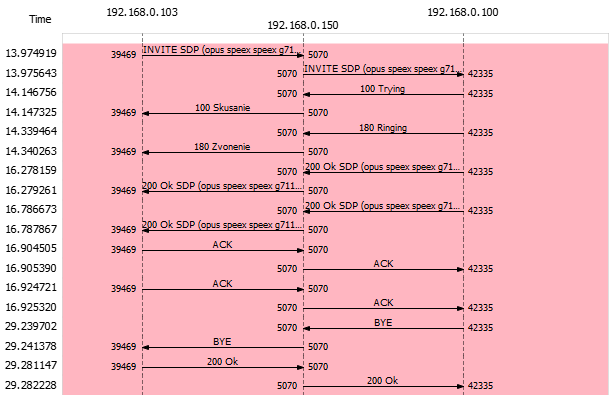
\includegraphics[scale=0.8]{Answered.png}
	\caption{Diagram hovoru medzi dvoma účastníkmi}
\end{figure}

Na tomto diagrame vidíme, že priebeh hovoru začína vždy požiadavkou \textbf{INVITE} od strany, ktorá chce hovor začať. V strede sa nachádza SIP Proxy Server, ktorý tút správu preposiela klientovi, ktorému je hovor určený. Následne z druhej strany vidíme odpoveď kódmi \textbf{100 Trying} a \textbf{180 Ringing}. Tu si môžeme všimnúť aj úspešné zmenenie znenia SIP kódov.

Ak to druhá strana zdvihne, pošle sa \textbf{200 OK} a následne na \textbf{200 OK} sa posiela potvrdzovacia správa \textbf{ACK}. V tomto momente sa hovor začal a medzi účastníkmi prebieha RTP / OPUS (UDP) komunikácia.

Zloženie hovoru funguje tak, že strana, ktorá chce zložiť pošle druhej strane správu \textbf{BYE}, ktorá je opätovne potvredná kódom \textbf{200 OK}. V tejto chvíli je hovor zrušený.

\begin{figure}[H]
	\centering
	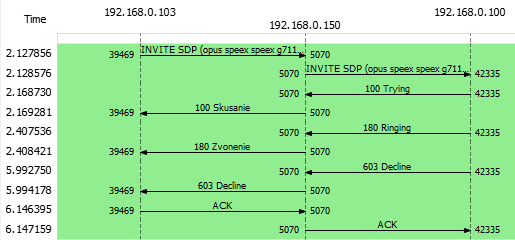
\includegraphics[scale=0.8]{Decline.png}
	\caption{Diagram hovoru, ktorý bol odmietnutý}
\end{figure}
Hovor, ktorý bol zrušený funguje rovnako ako normálny zdvihnutý hovor avšak na zmenu, že miesto poslania kódu \textbf{200 OK}, čím potvrdíme zdvihnutie sa posiela \textbf{603 Decline}, ktorá hovorí volajúcemu, že hovor bol zrušený (tzv. Obsadené).

\begin{figure}[H]
	\centering
	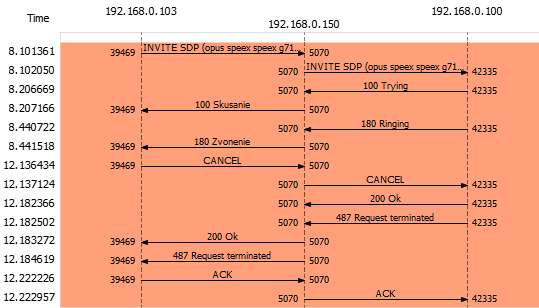
\includegraphics[scale=0.8]{Cancelled.png}
	\caption{Diagram hovoru, ktorý bol zrušený volajúcim}
\end{figure}
Zrušenie volajúcim funguje na podobnom princípe avšak ak volajúci zruší vytačanie druhej strane, volajúci pošle SIP požiadavku \textbf{CANCEL}, na ktorú je následne odpovedané \textbf{200 OK} ako potvrdenie a následne sa posiela \textbf{487 Request Terminated}. Volajúci ešte opútovne potvrdí správou \textbf{ACK}. Týmto bol hovor zrušený volajúcim a na druhej strane prestane vyzváňať telefón.

\subsection{Videohovor}
\begin{figure}[H]
	\centering
	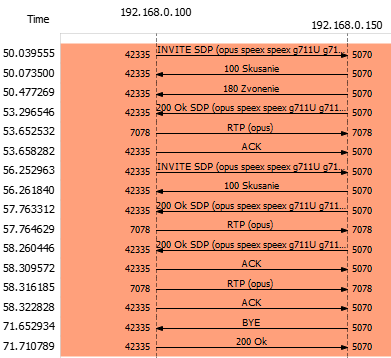
\includegraphics[scale=0.8]{Videocall.png}
	\caption{Diagram hovoru a následného pozvania k videohovoru}
\end{figure}
V tomto grafe nevidíme 3 strany ako v predchádzajúcich grafoch. NA tomto grafe vidíme iba volajúceho a server. Avšak požiadavky sú iba na druhú stranu zreplikované cez server.

Videohovor funguje na rovnakom princípe ako normálny hovor. Volajúci poslal najrpv \textbf{INVITE}, hovor sa prijal a začala \textbf{RTP} hlasová komunikácia medzi použovateľmi s definovanými kódekmi pre komunikáciu pomocou protokola \textbf{SDP}. Nateraz je medzi účastníkmi dohodnutý iba audio hovor, čiže aj kodeky, na ktorých sa dohodlo obsahujú iba audio kodeky.

Volajúci chcel v tomto prípade uskutočniť videohovor. Pre to sa znova poslal \textbf{INVITE} avšak už aj s video kodekmi. Audio komunikácia avšak stále prebieha, no ostatný proces je rovnaký ako keď sa počiatočne volá no bez správy \textbf{180 Ringing}. Následne po odpovedi \textbf{ACK} od volajúceho, ktorý chcel uskutočniť videohovor sa začína pomocou RTP prenášať aj video záznam s kamier klientov.

\subsection{Konferenčný hovor}
\begin{figure}[H]
	\centering
	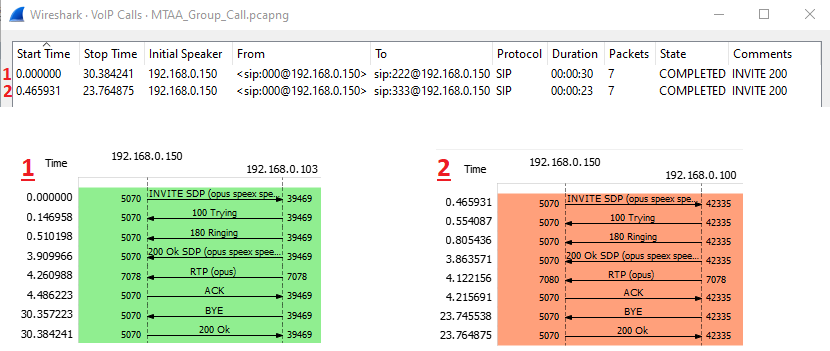
\includegraphics[scale=1, width=\textwidth]{Group.png}
	\caption{Diagram konferenčného hovoru}
\end{figure}
Konferenčný hovor prebieha ako dva samostatné normálne hovory. 
\subsection{Presmerovanie, podržanie}
\begin{figure}[H]
	\centering
	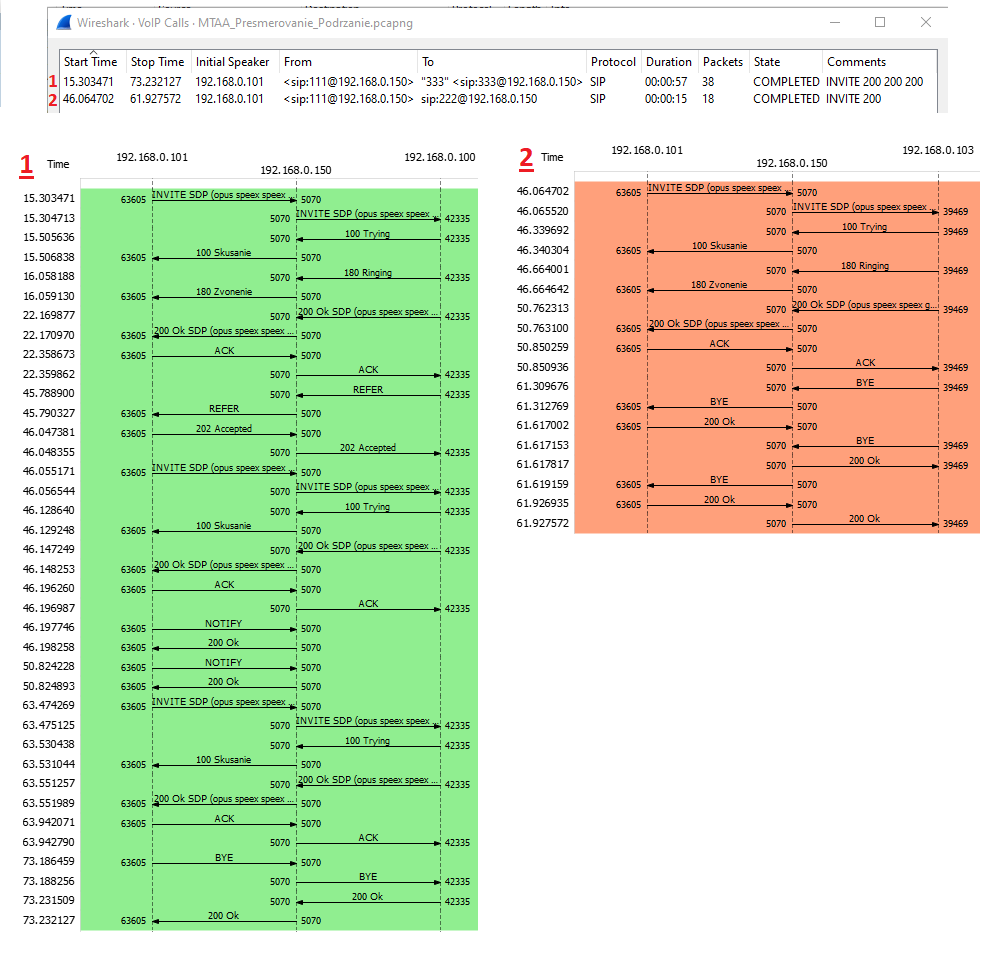
\includegraphics[scale=1, width=\textwidth]{ForwardHold.png}
	\caption{Diagram presmerovaného hovoru v rámci 3och klientov}
\end{figure}
Presmerovanie hovor funguje nasledovne. Klient, ktorý chce presmerovať spoluúčastníka hovoru na iné číslo, pošle správu \textbf{REFER}, ktorá hovorí o tom, že odkazujeme druhú stranu na iný kontakt. Druhá strana nám to akceptuje kódom \textbf{202 Accepted}. Následne budú medzi tymito klietnami prebiahť takzvané RE-INVITE, ktoré budú hovoriť o statuse v akom sa hovor nachádza. Po akceptovaní sa pošle \textbf{INVITE}, ktorý hovorí o tom, že hovor je podržaný. V prípade ak druhá strana ukončí hovor s novým kontaktom a navráti s ak nášmu hovoru pošle sa nový \textbf{INVITE}, ktorý hovorí o tom, že hovor sa navracia s podržania. 


\section{Záver}
V tomto zadaní sme si vyskúšali spojazdniť SIP telefónnu ústredňu pomocou extenrej knižnice. Riešenie zadania je funkčné a spĺňa všetky povinné funkcionality. Riešenie bolo overené pomocou programu Wireshark.  


\end{document}

%\begin{enumerate}[label=\textbf{\arabic*})]
%	\item X
%\end{enumerate}

%\begin{enumerate}[label=(\alph*)]
%	\item X
%\end{enumerate}

%\begin{figure}[H]
%	\centering
%	\includegraphics[scale=1, width=\textwidth]{FrameTypes.drawio.pdf}
%	\caption{Typy rámcov}
%\end{figure}